\documentclass[a4paper, 10pt, french]{article}

% Préambule; packages qui peuvent àªtre utiles
\usepackage[T1]{fontenc}        % Ce package pourrit les pdf...
\usepackage{babel,indentfirst}  % Pour les césures correctes,
                                       % et pour indenter au début de chaque paragraphe
\usepackage[utf8]{inputenc}   % Pour pouvoir utiliser directement les accents
                                     % et autres caractères français
\usepackage{lmodern,tgpagella} % Police de caractères
\textwidth 17cm \textheight 25cm \oddsidemargin -0.24cm % Définition taille de la page
\evensidemargin -1.24cm \topskip 0cm \headheight -1.5cm % Définition des marges

\usepackage{latexsym}                  % Symboles
\usepackage{amsmath}                   % Symboles mathématiques
\usepackage{tikz}   % Pour faire des schémas
\usepackage{graphicx} % Pour inclure des images
\usepackage{listings} % pour mettre des listings
% Fin Préambule; package qui peuvent àªtre utiles

\title{Rapport de TP 4MMSD : Conception d'un canal fiable à  partir de la couche UDP ainsi qu'un détecteur de fautes parfaits}
\author{ MAHIEU LUCAS étudiant PHELMA SLE 
\\ GONDOIS Pierre étudiant PHELMA SLE
}

\begin{document}

\maketitle

\section{Introduction}
Ce compte-rendu décrit le canal fiable et le détecteur de fautes du "TP Systèmes distribués". Pour ces deux points, nous présenterons dans un premier temps la spécification, les hypothèses posées, l'implémentation, puis l'évaluation du bon fonctionnement du produit.

\section{Canal fiable}

\subsection{Spécifications}
Le premier objectif du TP est d'implémenter un canal point-à -point dit "fiable" entre deux processus. L'interface processus / canal est composée de deux méthodes :

\begin{itemize}
	%actuellement ce n'est pas le cas
	\item send(m, p) : méthode permettant de charger au canal de livrer le message m au processus ayant le PID p. Cette méthode est accessible par les processus.
	\item deliver(m, p) : méthode permettant au canal de livrer le message m au processus p. Cette méthode est accessible par le canal.\newline
\end{itemize}
	
	Les garanties à  remplir par un canal "fiable" sont :
\begin{itemize}
	\item validité : si on processus correcte émet un message à  destination d'un processus correcte, alors ce dernier le délivrera.
	\item intégrité : un processus ne peut délivrer un message qu'au plus une fois et seulement ce message a été émis par un processus.
%question -> seulement ce message a été émis par un processus ??????  comprends pas 
\end{itemize}

\subsection{Hypothèses}
Les hypothèses qui ont été faites sur notre système sont ; 

\begin{itemize}
	\item Possibilité de panne franche de la part d'un ou des deux processus.
	\item Existence et utilisation d'un canal non fiable (UDP).
	\item Messages de longueur finie (longueur maximale de  (TBD ))
	\item Mémoire limitée. Les processus ne ont accès à  un espace mémoire fini.
	\item Ordre non garanti. L'ordre d'envoi des messages est différent de l'ordre de réception.
\end{itemize}


\subsection{Algorithme}
Nous allons décrire l'algorithme utilisé pour l'implémentation du canal fiable. Cette description se fera sous la forme de pseudo code. Les acteurs présents sont :
\begin{itemize}
	\item Le processus émetteur, maintenant appelé "processus A".
	\item L'extémité du canal à  qui le processus A a confié un message, maintenant appelé "canal A".
	\item L'extémité du canal à  qui le canal A a transmis un message, maintenant appelé "canal B".
	\item Le processus récepteur, maintenant appelé "processus B". \newline
\end{itemize}

\begin{figure}[!h]
\begin{center}
   	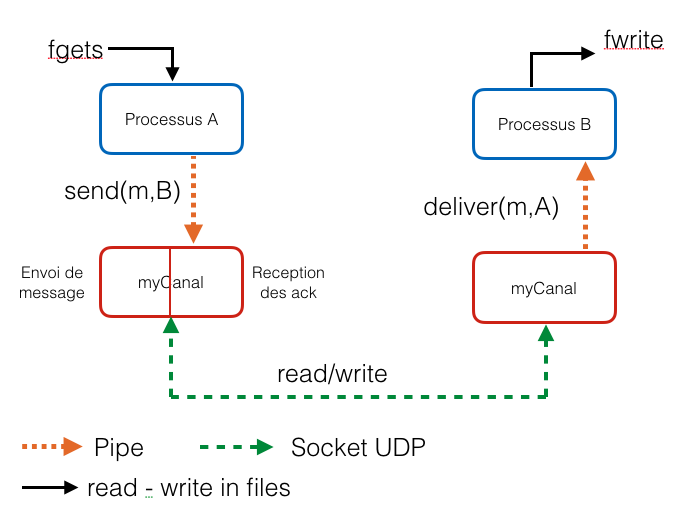
\includegraphics[scale=0.4]{exchange_stack.png}
	\caption{Schéma de fonctionnement du canal}
	\label{fig:canal}
\end{center}
\end{figure}

Fonctionnement du canal A :
Le canal A est composé de deux threads. Le premier est chargé d'envoyer les messages reçus de la part du processus A. Le deuxième réceptionne les messages d'acquittement de la part du canal B. En effet, lorsque le canal B reçoit un message de la part du canal A, il doit acquitter la réception du message auprès du canal A.

Processus de réception des messages : 

\subsection{Preuve}


\section{Détecteur de fautes}
\subsection{Spécifications}
Le détecteur de fautes est un processus qui a pour but de détecter les processus défectueux. Son fonctionnement repose sur le canal fiable. \newline
Le détecteur de faute établit une connection avec chacun des processus dont il veut vérifier le bon fonctionnement. Il envoie périodiquement des messages à ce processus dans l'attente d'une réponse. Si ce processus dans un temps imparti, alors le détecteur déclare ce processus comme disfonctionnel. \newline
Plusieurs états sont en fait possibles pour un processus qui ne répond pas. Le détecteur à fournir pour ce TP déclare un processus en "panne franche", ou "mort" s'il ne répond pas.

\subsection{Hypothèses}
Les hypothèses faites dans la réalisation du détecteur de fautes sont les suivantes :\newline
Si un processus ne répond pas au bout de 10 secondes, alors le processus à observer est déclaré mort. Le choix de 10 secondes n'est pas complètement arbitraire. Il n'y a jamais eu de manquement à cette borne si les deux processus étaient correctes. Les 10 secondes représentent une durée raisonnablement courte pour nos besoins. En effet, le délai de détection n'est utile que pour l'utilisateur.

\subsection{Algorithme}
Comme pour le canal fiable, 4 processus sont présents. Nous appèlerons processus C de détecteur de faute, et processus D le processus à observer. Les processus correspondants aux canaux de C et D sont lancés respectivement par les processus C et D. Nous ne détaillerons pas cela et partirons du principe que chacun des 4 processus existe pour expliquer le pseudo-code. Le canal possède un mode "détecteur de fautes"

Voici le pseudo-code des processus C et D : 
Processus C
% attention, les 10 secondes, le nombre de tour et la véracité sont à vérifier.
% Faire un schéma
while (1) {
	envoyer message au processus D (via le canal)
	attendre 10 secondes
	si un message a été reçu de la part du canal {
		afficher à l'utilisateur que D est en vie
	} sinon {
		déclarer la mort de D
		terminer le processus C et le canal C
	}
}


Processus D
while (1) {
	attendre message de la part du canal D, cette instruction est bloquante
	envoyer un message au canal D
}

Canal D
L'unique modification qui a été effectuée dans le canal D est l'ajout d'une instruction "read" bloquante avant d'envoyer un acquittement de message. En effet, le canal D doit vérifier que le processus D est bien en vie pour acquitter le message. Il attend donc que le processus D lui envoie un message. Ce message débloque le canal et lui permet d'envoyer cet acquittement.

Canal C:
La seule modification qui a été faite se trouve dans le thread de réception. La réception d'un acquittement, synonyme de bon fonctionnement du processus D, doit être transmise au processus C. A la réception d'un acquittement, le canal C transmet donc l'information au processus C, ce qui évite au processus C de considérer le processus D comme mort.

\subsection{Preuve}



\end{document}
